

\section{Topic Overview}
\label{section:overview}

Provide an overview of the topic to be studied...


\section{Objectives}
\label{section:objectives}

Explicitly state the objectives set to be achieved with this thesis...


\section{Thesis Outline}
\label{section:outline}

Briefly explain the contents of the different chapters...



\section{Theoretical Overview}
\label{section:overview}


Some overview of the underlying theory about the topic...


%%%%%%%%%%%%%%%%%%%%%%%%%%%%%%%%%%%%%%%%%%%%%%%%%%%%%%%%%%%%%%%%%%%%%%%%
\section{Theoretical Model 1}
\label{section:theory1}



Multiple citations are compressed when using the {\tt sort\&compress} option when loading the {\tt natbib} package as {\tt \textbackslash usepackage[numbers,sort\&compress]\{natbib\}} in file {\tt Thesis\_Preamble.tex}, resulting in citations like ~\citep{Hull,Wilmott}.


%%%%%%%%%%%%%%%%%%%%%%%%%%%%%%%%%%%%%%%%%%%%%%%%%%%%%%%%%%%%%%%%%%%%%%%%
\section{Theoretical Model 2}
\label{section:theory2}

Other models...




Insert your chapter material here...

%%%%%%%%%%%%%%%%%%%%%%%%%%%%%%%%%%%%%%%%%%%%%%%%%%%%%%%%%%%%%%%%%%%%%%%%
\section{Numerical Model}
\label{section:model}

Description of the numerical implementation of the models explained in Chapter~\ref{chapter:background}...


%%%%%%%%%%%%%%%%%%%%%%%%%%%%%%%%%%%%%%%%%%%%%%%%%%%%%%%%%%%%%%%%%%%%%%%%
\section{Verification and Validation}
\label{section:verification}

Basic test cases to compare the implemented model against other numerical tools (verification) and experimental data (validation)...



Insert your chapter material here...


%%%%%%%%%%%%%%%%%%%%%%%%%%%%%%%%%%%%%%%%%%%%%%%%%%%%%%%%%%%%%%%%%%%%%%%%
\section{Problem Description}
\label{section:problem}

Description of the baseline problem...


%%%%%%%%%%%%%%%%%%%%%%%%%%%%%%%%%%%%%%%%%%%%%%%%%%%%%%%%%%%%%%%%%%%%%%%%
\section{Baseline Solution}
\label{section:baseline}

Analysis of the baseline solution...


%%%%%%%%%%%%%%%%%%%%%%%%%%%%%%%%%%%%%%%%%%%%%%%%%%%%%%%%%%%%%%%%%%%%%%%%
\section{Enhanced Solution}
\label{section:enhanced}

Quest for the optimal solution...


% ----------------------------------------------------------------------
\subsection{Figures}
\label{subsection:figures}

Insert your section material and possibly a few figures...

Make sure all figures presented are referenced in the text!


% ----------------------------------------------------------------------
\subsubsection{Images}
\label{subsection:images}

\iffalse
\begin{figure}[!htb]
  \centering
  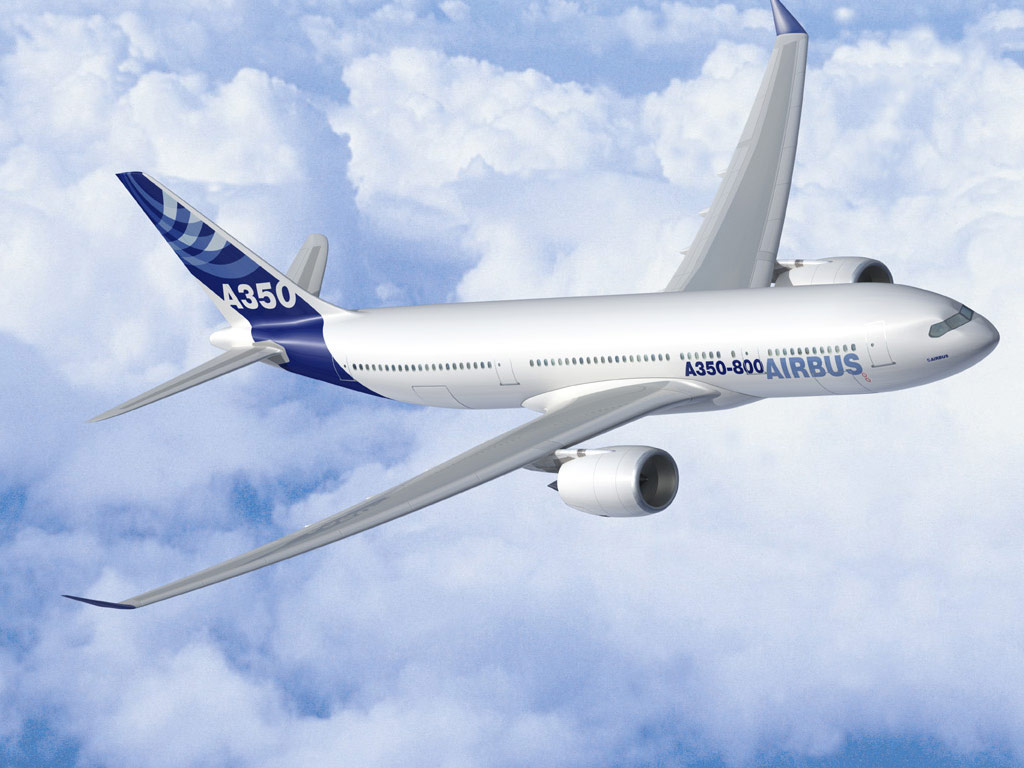
\includegraphics[width=0.25\textwidth]{Airbus_A350.jpg}
  \caption[Caption for figure in TOC.]{Caption for figure.}
  \label{fig:airbus1}
\end{figure}

\begin{figure}[!htb]
  \begin{subfigmatrix}{2}
    \subfigure[Airbus A320]{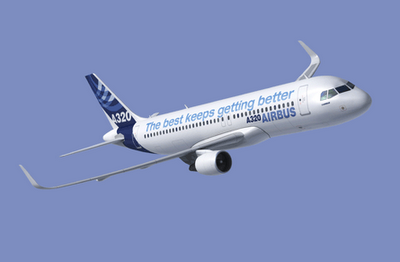
\includegraphics[width=0.49\linewidth]{Airbus_A320_sharklets.png}}
    \subfigure[Bombardier CRJ200]{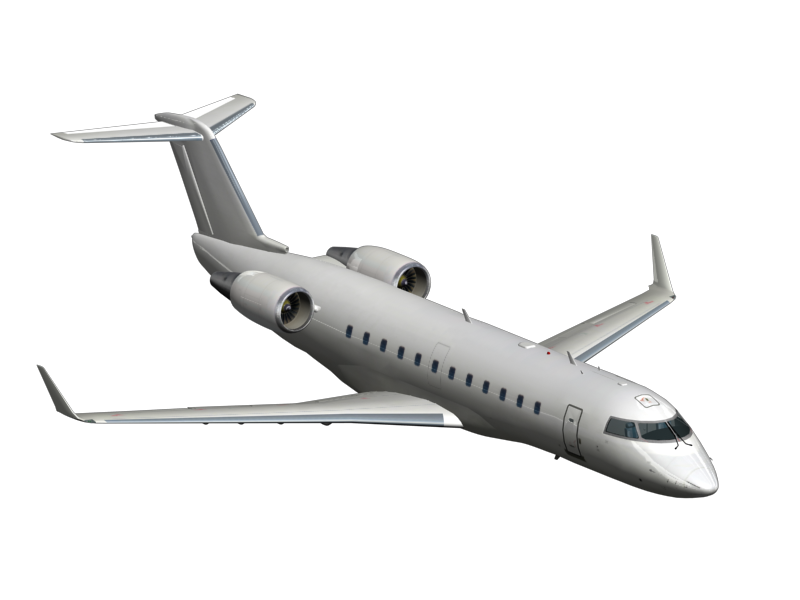
\includegraphics[width=0.49\linewidth]{Bombardier_CRJ200.png}}
  \end{subfigmatrix}
  \caption{Some aircrafts.}
  \label{fig:aircrafts}
\end{figure}
\fi

Make reference to Figures \ref{fig:airbus1} and \ref{fig:aircrafts}.

By default, the supported file types are {\it .png,.pdf,.jpg,.mps,.jpeg,.PNG,.PDF,.JPG,.JPEG}.

See \url{http://mactex-wiki.tug.org/wiki/index.php/Graphics_inclusion} for adding support to other extensions.


% ----------------------------------------------------------------------
\subsubsection{Drawings}
\label{subsection:drawings}

Insert your subsection material and for instance a few drawings...

The schematic illustrated in Fig.~\ref{fig:algorithm} can represent some sort of algorithm.
\iffalse
\begin{figure}[!htb]
  \centering
  \scriptsize
%  \footnotesize 
%  \small
  \setlength{\unitlength}{0.9cm}
  \begin{picture}(8.5,6)
    \linethickness{0.3mm}

    \put(3,6){\vector(0,-1){1}}
    \put(3.5,5.4){$\bf \alpha$}
    \put(3,4.5){\oval(6,1){}}
    %\put(0,4){\framebox(6,1){}}
    \put(0.3,4.4){Grid Generation: \quad ${\bf x} = {\bf x}\left({\bf \alpha}\right)$}

    \put(3,4){\vector(0,-1){1}}
    \put(3.5,3.4){$\bf x$}
    \put(3,2.5){\oval(6,1){}}
    %\put(0,2){\framebox(6,1){}}
    \put(0.3,2.4){Flow Solver: \quad ${\cal R}\left({\bf x},{\bf q}\left({\bf x}\right)\right) = 0$}

    \put(6.0,2.5){\vector(1,0){1}}
    \put(6.4,3){$Y_1$}

    \put(3,2){\vector(0,-1){1}}
    \put(3.5,1.4){$\bf q$}
    \put(3,0.5){\oval(6,1){}}
    %\put(0,0){\framebox(6,1){}}
    \put(0.3,0.4){Structural Solver: \quad ${\cal M}\left({\bf x},{\bf q}\left({\bf x}\right)\right) = 0$}

    \put(6.0,0.5){\vector(1,0){1}}
    \put(6.4,1){$Y_2$}

    %\put(7.8,2.5){\oval(1.6,5){}}
    \put(7.0,0){\framebox(1.6,5){}}
    \put(7.1,2.5){Optimizer}
    \put(7.8,5){\line(0,1){1}}
    \put(7.8,6){\line(-1,0){4.8}}
  \end{picture}
  \caption{Schematic of some algorithm.}
  \label{fig:algorithm}
\end{figure}
\fi

% ----------------------------------------------------------------------
\subsection{Equations}
\label{subsection:equations}

Equations can be inserted in different ways.

The simplest way is in a separate line like this

\begin{equation}
  \frac{{\rm d} q_{ijk}}{{\rm d} t} + {\cal R}_{ijk}({\bf q}) = 0 \,.
\label{eq:ode}
\end{equation}

If the equation is to be embedded in the text. One can do it like this ${\partial {\cal R}}/{\partial {\bf q}}=0$.

It may also be split in different lines like this
\iffalse
\begin{eqnarray}
  {\rm Minimize}   && Y({\bf \alpha},{\bf q}({\bf \alpha}))            \nonumber           \\
  {\rm w.r.t.}     && {\bf \alpha} \,,                                 \label{eq:minimize} \\
  {\rm subject~to} && {\cal R}({\bf \alpha},{\bf q}({\bf \alpha})) = 0 \nonumber           \\
                   &&       C ({\bf \alpha},{\bf q}({\bf \alpha})) = 0 \,. \nonumber
\end{eqnarray}

It is also possible to use subequations. Equations~\ref{eq:continuity}, \ref{eq:momentum} and \ref{eq:energy} form the Naver--Stokes equations~\ref{eq:NavierStokes}.

\begin{subequations}
    \begin{equation}
    \frac{\partial \rho}{\partial t} + \frac{\partial}{\partial x_j}\left( \rho u_j \right) = 0 \,,
    \label{eq:continuity}
    \end{equation}
    \begin{equation}
    \frac{\partial}{\partial t}\left( \rho u_i \right) + \frac{\partial}{\partial x_j} \left( \rho u_i u_j + p \delta_{ij} - \tau_{ji} \right) = 0, \quad i=1,2,3 \,,
    \label{eq:momentum}
    \end{equation}
    \begin{equation}
        \frac{\partial}{\partial t}\left( \rho E \right) + \frac{\partial}{\partial x_j} \left( \rho E u_j + p u_j - u_i \tau_{ij} + q_j \right) = 0 \,.
    \label{eq:energy}
    \end{equation}
\label{eq:NavierStokes}%
\end{subequations}
\fi

% ----------------------------------------------------------------------
\subsection{Tables}
\label{section:tables}

Insert your subsection material and for instance a few tables...

Make sure all tables presented are referenced in the text!

Follow some guidelines when making tables:
\iffalse
\begin{itemize}
  \item Avoid vertical lines
  \item Avoid “boxing up” cells, usually 3 horizontal lines are enough: above, below, and after heading
  \item Avoid double horizontal lines
  \item Add enough space between rows
\end{itemize}

\begin{table}[!htb]
  \renewcommand{\arraystretch}{1.2} % more space between rows
  \centering
  \begin{tabular}{lccc}
    \toprule
    Model           & $C_L$ & $C_D$ & $C_{M y}$ \\
    \midrule
    Euler           & 0.083 & 0.021 & -0.110    \\
    Navier--Stokes  & 0.078 & 0.023 & -0.101    \\
    \bottomrule
  \end{tabular}
  \caption[Table caption shown in TOC.]{Table caption.}
  \label{tab:aeroCoeff}
\end{table}

Make reference to Table \ref{tab:aeroCoeff}.

Tables \ref{tab:memory} and \ref{tab:multipleColumns} are examples of tables with merging columns:

\begin{table}[!htb]
  \renewcommand{\arraystretch}{1.2} % more space between rows
  \centering
  \begin{tabular}[]{lrr}
    \toprule
                & \multicolumn{2}{c}{\underline{Virtual memory [MB]}} \\
                & Euler       & Navier--Stokes \\
    \midrule
      Wing only &  1,000      &    2,000       \\
      Aircraft  &  5,000      &   10,000       \\
      (ratio)   & $5.0\times$ & $5.0\times$    \\
    \bottomrule
  \end{tabular}
  \caption{Memory usage comparison (in MB).}
  \label{tab:memory}
\end{table}

\begin{table}[!htb]
  \centering
  \renewcommand{\arraystretch}{1.2} % more space between rows
  \begin{tabular}{@{}rrrrcrrr@{}} % remove space to the vertical edges @{}...@{}
    \toprule
      & \multicolumn{3}{c}{$w = 2$} & \phantom{abc} & \multicolumn{3}{c}{$w = 4$} \\
    \cmidrule{2-4}
    \cmidrule{6-8}
      & $t=0$ & $t=1$ & $t=2$ && $t=0$ & $t=1$ & $t=2$ \\
    \midrule
      $dir=1$
      \\
      $c$ &  0.07 &  0.16 &  0.29 &&  0.36 &  0.71 &   3.18 \\
      $c$ & -0.86 & 50.04 &  5.93 && -9.07 & 29.09 &  46.21 \\
      $c$ & 14.27 &-50.96 &-14.27 && 12.22 &-63.54 &-381.09 \\
      $dir=0$
      \\
      $c$ &  0.03 &  1.24 &  0.21 &&  0.35 & -0.27 &  2.14 \\
      $c$ &-17.90 &-37.11 &  8.85 &&-30.73 & -9.59 & -3.00 \\
      $c$ &105.55 & 23.11 &-94.73 &&100.24 & 41.27 &-25.73 \\
    \bottomrule
  \end{tabular}
  \caption{Another table caption.}
  \label{tab:multipleColumns}
\end{table}

An example with merging rows can be seen in Tab.\ref{tab:multipleRows}.

\begin{table}[!htb]
  \renewcommand{\arraystretch}{1.2} % more space between rows
  \centering
  \begin{tabular}{ccccc}
    \toprule
      \multirow{2}{*}{ABC} & \multicolumn{4}{c}{header} \\
      \cmidrule{2-5} & 1.1 & 2.2 & 3.3 & 4.4 \\
    \midrule
      \multirow{2}{*}{IJK} & \multicolumn{2}{c}{\multirow{2}{*}{group}} & 0.5 & 0.6 \\
      \cmidrule{4-5}       & \multicolumn{2}{c}{}                       & 0.7 & 1.2 \\
    \bottomrule
  \end{tabular}
  \caption{Yet another table caption.}
  \label{tab:multipleRows}
\end{table}

If the table has too many columns, it can be scaled to fit the text widht, as in Tab.\ref{tab:scale}.
\begin{table}[!htb]
  \renewcommand{\arraystretch}{1.2} % more space between rows
  \centering
  \resizebox*{\textwidth}{!}{%
    \begin{tabular}[]{lcccccccccc}
      \toprule
        Variable &  a  &  b  &  c  &  d  &  e  &  f  &  g  &  h  &  i  &  j  \\
      \midrule
        Test 1   &  10,000 &  20,000 &  30,000 &  40,000 &  50,000 &  60,000 &  70,000 &  80,000 &  90,000 & 100,000 \\
        Test 2   &  20,000 &  40,000 &  60,000 &  80,000 & 100,000 & 120,000 & 140,000 & 160,000 & 180,000 & 200,000 \\
      \bottomrule
    \end{tabular}
  }%
  \caption{Very wide table.}
  \label{tab:scale}%
\end{table}
\fi

% ----------------------------------------------------------------------
\subsection{Mixing}
\label{section:mixing}

If necessary, a figure and a table can be put side-by-side as in Fig.\ref{fig:side_by_side}
\iffalse
\begin{figure}[!htb]
  \begin{minipage}[b]{0.60\linewidth}
    \centering
    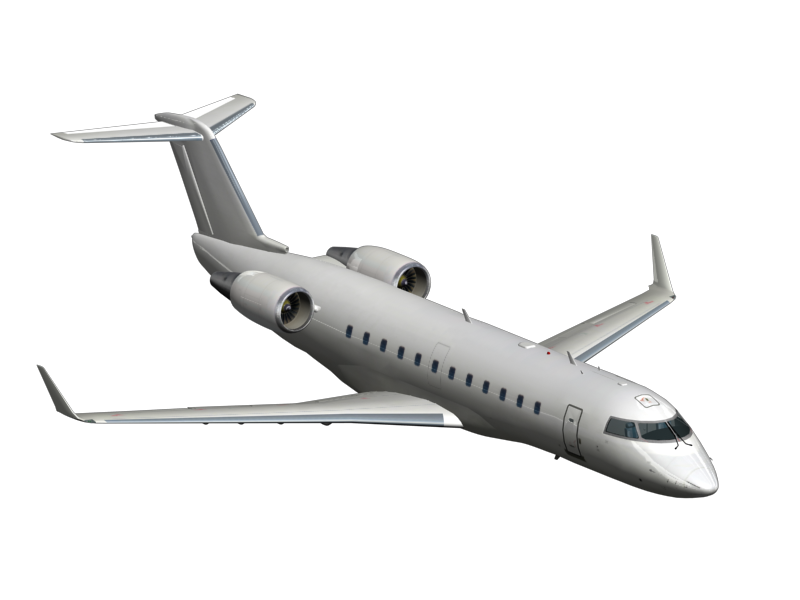
\includegraphics[width=\linewidth]{Bombardier_CRJ200}
  \end{minipage}%
  \begin{minipage}[b]{0.30\linewidth}
    \centering
    \begin{tabular}[b]{lll}
      \toprule
        \multicolumn{3}{c}{Legend} \\
      \midrule
        A & B & C \\
        0 & 0 & 0 \\
        0 & 1 & 0 \\
        1 & 0 & 0 \\
        1 & 1 & 1 \\
      \bottomrule
    \end{tabular}
    \vspace{5em}
  \end{minipage}
\caption{Figure and table side-by-side.}
\label{fig:side_by_side}
\end{figure}

\fi

Insert your chapter material here...


% ----------------------------------------------------------------------
\section{Achievements}
\label{section:achievements}

The major achievements of the present work...


% ----------------------------------------------------------------------
\section{Future Work}
\label{section:future}

A few ideas for future work...


% ----------------------------------------------------------------------
In case an appendix if deemed necessary, the document cannot exceed a total of 100 pages...

Some definitions and vector identities are listed in the section below.
\section{Vector identities}
\label{section:vectorIdentities}

\begin{equation}
	\nabla \times \left( \nabla \phi \right) = 0
	\label{eq:cross_nnp}
\end{equation}

\begin{equation}
	\nabla \cdot \left( \nabla \times {\bf u} \right) = 0
	\label{eq:dotCross_nnu}
\end{equation}
